\documentclass[10pt,a4paper]{article}
\usepackage[a4paper,left=2.0cm,right=2.0cm,top=2.1cm,bottom=2.2cm,headheight=13pt]{geometry}
\usepackage[T1]{fontenc}
\usepackage[utf8]{inputenc}
\usepackage{mathpazo}
\usepackage[scaled=0.92]{helvet}
\usepackage{microtype}
\usepackage{amsmath,amssymb,bm}
\usepackage{booktabs,tabularx,array,multirow}
\usepackage[table]{xcolor}
\usepackage{graphicx}
\usepackage{enumitem}
\usepackage{titlesec}
\usepackage{fancyhdr}
\usepackage[most]{tcolorbox}
\usepackage[authoryear,round,sort]{natbib}
\usepackage{tikz}
\usetikzlibrary{arrows.meta,positioning,shapes.geometric,fit,backgrounds,calc}
\usepackage{caption}
\usepackage[colorlinks=true,linkcolor=navy,citecolor=navy,urlcolor=navy]{hyperref}

\hypersetup{pdftitle={FORACCA 2.0: technical concept and methodological specification},pdfauthor={Narek Ohanyan},pdfsubject={A hybrid process--statistical framework for climate-smart reforestation in Armenia}}
\definecolor{navy}{HTML}{16365C}
\definecolor{teal}{HTML}{0F766E}
\definecolor{rust}{HTML}{B4491F}
\definecolor{sand}{HTML}{F4EFE6}
\definecolor{mist}{HTML}{EAF0F6}
\definecolor{slate}{HTML}{4B5563}
\definecolor{okgreen}{HTML}{D9EFE3}
\definecolor{okamber}{HTML}{FBF0CF}
\definecolor{okred}{HTML}{F6DAD3}

\setlength{\parskip}{3.2pt plus 1pt}
\setlength{\parindent}{0pt}
\linespread{1.02}
\setlist{nosep,leftmargin=1.3em,itemsep=1.5pt}
\numberwithin{equation}{section}
\captionsetup{font=small,labelfont={bf,sf},labelsep=period,justification=raggedright,singlelinecheck=false}
\setlength{\abovecaptionskip}{4pt}
\setlength{\belowcaptionskip}{2pt}
\setlength{\floatsep}{8pt plus 2pt minus 2pt}
\setlength{\textfloatsep}{9pt plus 2pt minus 3pt}
\setlength{\intextsep}{8pt plus 2pt minus 2pt}
\setlength{\abovedisplayskip}{5pt plus 1pt minus 2pt}
\setlength{\belowdisplayskip}{5pt plus 1pt minus 2pt}
\renewcommand{\arraystretch}{1.12}
\bibsep=1.4pt
\setlength{\bibhang}{1.2em}

\titleformat{\section}{\Large\sffamily\bfseries\color{navy}}{\thesection}{0.6em}{}
\titleformat{\subsection}{\normalsize\sffamily\bfseries\color{navy}}{\thesubsection}{0.5em}{}
\titleformat{\subsubsection}[runin]{\normalsize\sffamily\bfseries\color{slate}}{}{0em}{}[.\ ]
\titlespacing*{\section}{0pt}{11pt plus 2pt minus 2pt}{4pt}
\titlespacing*{\subsection}{0pt}{7pt plus 2pt minus 1pt}{2pt}
\titlespacing*{\subsubsection}{0pt}{3pt}{0.4em}

\pagestyle{fancy}
\fancyhf{}
\renewcommand{\headrulewidth}{0.3pt}
\fancyhead[L]{\footnotesize\sffamily\color{slate}FORACCA 2.0 \textperiodcentered\ technical concept and methodological specification}
\fancyhead[R]{\footnotesize\sffamily\color{slate}Draft v2.0 \textperiodcentered\ 21 September 2026}
\fancyfoot[C]{\footnotesize\sffamily\thepage}

% ---- shorthand
\newcommand{\Hmin}{H_{\min}}
\newcommand{\hmech}{h^{\text{mech}}}
\newcommand{\hstat}{h^{\text{stat}}}
\newcommand{\PLC}{\mathrm{PLC}}
\newcommand{\HFI}{\mathrm{HFI}}
\newcommand{\VPD}{\mathrm{VPD}}
\newcommand{\CWD}{\mathrm{CWD}}
\newcommand{\WSI}{\mathrm{WSI}}
\newcommand{\REW}{\mathrm{REW}}
\newcommand{\DI}{\mathrm{DI}}
\newcommand{\cloglog}{\operatorname{cloglog}}
\newcommand{\E}{\mathbb{E}}
\newcommand{\Prob}{\mathbb{P}}
\newcommand{\ind}{\mathbb{1}}
\newcommand{\note}[1]{\textcolor{rust}{\textbf{#1}}}

\newtcolorbox{keybox}[1][]{enhanced,breakable,colback=sand,colframe=navy!70,boxrule=0.5pt,arc=1.5pt,left=6pt,right=6pt,top=4pt,bottom=4pt,fonttitle=\sffamily\bfseries\small,#1}

\begin{document}

\thispagestyle{plain}
{\raggedright
{\sffamily\bfseries\Huge\color{navy} FORACCA 2.0}\\[3pt]
{\sffamily\bfseries\Large A hybrid process--statistical framework for predicting where climate-resilient reforestation will hold in Armenia}\\[4pt]
{\sffamily\small\color{slate} Technical concept and methodological specification \textperiodcentered\ successor to Output~1.2 (v1, 16~March 2026)}\\[3pt]
{\sffamily\small Narek Ohanyan \textperiodcentered\ Acopian Center for the Environment, American University of Armenia \textperiodcentered\ Draft v2.0, 21~September 2026}\par}
\vspace{4pt}
\hrule height 0.6pt
\vspace{6pt}

\begin{tcolorbox}[enhanced,colback=mist,colframe=mist,boxrule=0pt,arc=1.5pt,left=7pt,right=7pt,top=5pt,bottom=5pt]
\textbf{\sffamily Abstract.} Version~1 of the FORACCA vulnerability model asked a random forest to reproduce the local spread of canopy height from three climate deltas, and then read the answer as a forecast. Re-running its own training table shows why that cannot work: the model scores $R^2=0.29$ on a random split and $R^2=0.04$ when whole 25~km blocks are held out, while on the same random split a forest given only longitude and latitude scores 0.45. Beyond the training range its output is constant. Version~2 replaces the score with an estimand that can be tested, the probability $V$ that a planted cohort survives and reaches canopy height under a stated climate trajectory, and builds it from five coupled modules: topoclimate and water balance; a two-phase plant-hydraulic failure engine; a panel discrete-time hazard model fitted to observed dieback; an adult-niche, attainable-height, growth and establishment module; and a competing-risk viability integrator feeding a CVaR-robust planting portfolio. Physics decides where observations cannot, observations decide where physics is uncertain, and an area-of-applicability gate arbitrates between them. The validation protocol is fixed before fitting, uncertainty is partitioned rather than summarised, and the core formulas below are implemented and unit-tested in the accompanying Python skeleton.
\end{tcolorbox}

\vspace{2pt}
\begin{keybox}[title={What changes from version 1 to version 2}]
\small
\renewcommand{\arraystretch}{1.14}
\begin{tabularx}{\linewidth}{@{}>{\sffamily\bfseries}p{2.45cm}>{\raggedright\arraybackslash}X>{\raggedright\arraybackslash}X@{}}
 & \textbf{\sffamily Version 1} & \textbf{\sffamily Version 2}\\[1pt]
\hline
Target & A vulnerability index (FVS) built from climate deltas scaled by the spread of canopy height & Cohort viability $V$: probability that planted trees survive and reach $\Hmin$ under trajectory $\omega$\\
Climate & Epoch-mean deltas, one model, 1~km & Daily forcing, 5+ GCMs $\times$ 4 SSPs, trend-preserving downscaling to 30~m topoclimate; VPD built last from dew-point-downscaled humidity\\
Physiology & Absent & Two-phase hydraulic failure: stomatal closure, then cuticular loss with a $g_{\min}$ heat phase transition\\
Observations & One static canopy-height statistic on forest-mask survivors & Annual dieback events and tree-ring growth collapses for every forest pixel present at the start, censored by harvest and fire\\
Learning & Random 80/20 split, random forest, Gini importances used as coefficients & Spatial-block, forward-chaining, leave-province-out and extrapolation CV; proper scores; monotone GLM/GBM stack; conformal intervals\\
Extrapolation & Silent: output is flat outside the training range & Explicit: area-of-applicability gate hands over to the mechanistic hazard\\
Forest ecology & Absent & Establishment hazard, attainable height, growth in physiological age, stand coupling through leaf area, adult niche as consistency test\\
Uncertainty, decision & One realisation; no decision layer & Factorial ensemble with variance partitioning; CVaR-robust species--site portfolio\\
\end{tabularx}
\end{keybox}

\section{What version 1 taught us}\label{sec:audit}

The v1 note defined a forest vulnerability score, $\mathrm{FVS}=\int(\alpha\,\Delta\VPD+\beta\,\Delta T_{\max}-\gamma\,\Delta P)\,\sigma(H)^{-1}\,dt$, with $\alpha,\beta,\gamma$ to be read off random-forest importances, and the repository trained a random forest to predict $\sigma(H)$, the local standard deviation of canopy height, from three growing-season climate deltas on 4\,338 one-kilometre pixels. A Streamlit app then added scenario deltas to the table and reported the shortfall of predicted against observed $\sigma(H)$ as vulnerability. It is a working end-to-end prototype, which is exactly why we can be specific about what has to change. We re-ran the delivered table and model (\texttt{scripts/audit\_v1.py}; the hyper-parameters, seed and split reproduce the published $R^2=0.292$ and MAE $=1.80$~m exactly), and Table~\ref{tab:audit} lists what we found.

\begin{table}[t]
\centering
\caption{Audit of the v1 training table and model. All numbers are recomputed from \texttt{Armenia\_ML\_Training\_Data.parquet} ($n=4\,338$ pixels; RF: 500 trees, depth 15, seed 42).}\label{tab:audit}
\footnotesize
\renewcommand{\arraystretch}{1.1}
\begin{tabularx}{\linewidth}{@{}>{\raggedright\arraybackslash\bfseries\sffamily}p{2.55cm}>{\raggedright\arraybackslash}X>{\raggedright\arraybackslash}p{4.6cm}@{}}
\toprule
Finding & Evidence & Consequence for v2\\
\midrule
Validation leaks space & Random 80/20 split: $R^2=0.29$, MAE 1.80~m (predicting the mean: 2.13~m). Blocked 5-fold CV: $R^2=0.20,\,0.11,\,0.04,\,-0.28,\,-0.45$ for 5, 10, 25, 50, 75~km blocks. Median nearest-neighbour spacing 0.7~km; neighbours correlate at $r=0.97$--$0.997$ in every feature and 0.58 in the target. & Skill was interpolation between near-duplicates. Block size must come from the data and the CV must mimic the use (\S\ref{sec:ml}).\\
The features are coordinates & The three deltas predict longitude and latitude with $R^2=0.87$ and $0.89$. Longitude and latitude alone reach $R^2=0.45$ on the same random split, and $-0.06$ at 25~km blocks against 0.04 for the climate features. & A climate model must beat a coordinates-only baseline under blocked CV, or it has learned nothing about climate.\\
Extrapolation is a constant & Training range of $\Delta T_{\max}$ is 0.05--0.10~K. Adding any warming $\ge 0.25$~K changes no prediction (max difference $4\times10^{-16}$~m). Mean FVS is 60.6\,\% for SSP1-2.6 mid-century and 64.6\,\% for SSP5-8.5 end-century, against 6.6\,\% with deltas as observed: the mildest scenario already produces 54 of the 58 points by which the harshest exceeds the no-forcing baseline (Fig.~\ref{fig:v1}b). & Outside the training support the model must hand over to physics, and say so (\S\ref{sec:gate}).\\
The label measures structure & $\sigma(H)$ is predicted from mean height alone with $R^2=0.67$; its median coefficient of variation is 0.58. At 1~km it mostly reflects cover fraction and stand mosaic, not physiological stress. & The response must be an event that happened to a tree or stand (dieback, growth collapse, planting failure).\\
Importances are not coefficients & Gini importances are 34.9, 31.4 and 33.7\,\% for VPD, $T_{\max}$ and $P$: near-equal, unsigned, and taken from a model that cannot extrapolate. They were described as SHAP values and proposed as $\alpha,\beta,\gamma$. & Effects come from a hazard model with signs and units; ALE and SHAP are used to explain, never to parametrise.\\
Units and construction & $\Delta\VPD/\Delta T_{\max}=0.83$~kPa~K$^{-1}$ in the table; at fixed relative humidity it should be 0.03--0.25. Training VPD (CHELSA) and scenario VPD (CMIP6-derived) are built differently, and the deltas themselves are small (mean $\Delta T_{\max}=0.07$~K). & One VPD construction end to end, checked by a thermodynamic unit test (\S\ref{sec:A}).\\
No time, no events, survivors only & One row per pixel; no year, no exposure, no mortality event. The forest mask conditions on persistence, so pixels that died are excluded by construction. & Event histories for every pixel that was forest at the start, with harvest and fire as competing events (\S\ref{sec:C}).\\
Score $\neq$ formula & The app evaluates $\mathrm{clip}\big((\sigma_{\text{obs}}-\sigma_{\text{pred}})/\sigma_{\text{obs}}\times100,0,100\big)$, a model residual, not the time integral of the concept note. & Estimand defined once, in probability units (\S\ref{sec:estimand}).\\
\bottomrule
\end{tabularx}
\end{table}

\begin{figure}[t]
\centering
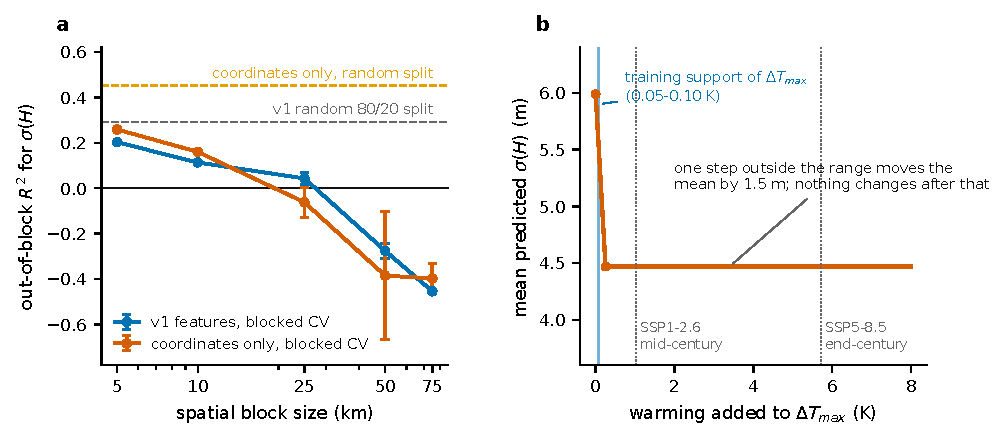
\includegraphics[width=\linewidth]{fig1_v1_audit.pdf}
\caption{The v1 model, audited on its own data. (a) Out-of-block $R^2$ against block size for the v1 features (blue) and for coordinates alone (vermilion); dashed lines show the random-split scores. Points are means of three block assignments, bars $\pm$1~SD. (b) Mean predicted $\sigma(H)$ as extra warming is added to $\Delta T_{\max}$ with the other two deltas unchanged: one step outside the training range moves the mean by 1.5~m and nothing moves it afterwards.}\label{fig:v1}
\end{figure}

None of this diminishes what v1 achieved. It settled the data plumbing, the raster conventions, and a demonstrable interface, and it made the central problem legible: when a model is trained on the spatial pattern of a static quantity, it learns geography, and geography does not project. Everything that follows is designed to make that failure impossible to repeat, and to replace a single number with a chain of quantities that can each be checked against something observable.

\section{Question, estimand and design principles}\label{sec:design}

\subsection{Where the field stands, and what Armenia already tells us}
Drought- and heat-induced tree mortality has been documented across forested biomes worldwide \citep{Allen2010} and is understood well enough mechanistically that it should not be estimated from correlations alone. Syntheses converge on hydraulic failure, often compounded by carbon limitation and biotic attack, as the proximate cause across biomes \citep{McDowell2008,Adams2017,Choat2018,Hartmann2018}, and xylem safety margins are strikingly convergent across forests \citep{Choat2012}. Two recent results sharpen this for our purposes. First, survival time under drought is a two-phase process: stomatal closure delays failure, after which the tree drains its own storage through the cuticle, and in a 16-species temperate experiment the first phase accounted for 85--97\,\% of total survival time \citep{Waite2026,Gauthey2026}, in line with the earlier argument that timely stomatal closure governs resistance \citep{MartinStPaul2017}. Second, the minimum leaf conductance $g_{\min}$ is not a constant: it rises steeply above a species-specific temperature \citep{Cochard2019,Duursma2019}, which is why heat waves can kill trees that drought alone would not. Trait-based hydraulic models such as SurEau \citep{Cochard2021,Ruffault2022} embody these ideas, but they need parameters we do not have for Caucasian species, and their probabilities have never been calibrated against Armenian mortality.

The correlative alternative, species distribution models fitted to occurrence, is what most Caucasus studies use \citep{Pshegusov2022,Dagtekin2020}. It tells us where species are under present climate; it rests on an equilibrium assumption and leaves out demography and dispersal \citep{Guisan2005}; it is known to fail under non-analogue conditions \citep{Pearson2003,Fitzpatrick2009,Elith2010}, and it says nothing about whether a planted seedling survives its first summers. The productive middle path is hybrid: mechanism supplies the functional form outside the observed range, data supply calibration inside it \citep{Kearney2009,Reichstein2019}.

Local evidence defines what the framework must reproduce. In southern Armenia the mean ring width of \emph{Fagus orientalis} at Shikahogh fell from 1.95~mm in 1965--1993 to 0.89~mm in 1994--2023, with no natural regeneration, while at the northern stand of Teghut it rose from 1.67 to 2.14~mm; local warming runs at 0.026--0.032\,$^\circ$C per year \citep{Stepanyan2026}. Oak and beech in Tavush lose growth and theoretical hydraulic conductivity in extreme dry years and recover within two years, beech faster \citep{Voss2025}; junipers at Khosrov are more drought-sensitive than oak at Tezharuyk \citep{OpalaOwczarek2021}. Caucasian distributions are governed by topography and water regime \citep{Pshegusov2022}, and \emph{F.~orientalis} is projected to contract sharply with the Caucasus retained as refugium \citep{Dagtekin2020}. These are patterns the calibrated model must pass, not decoration (\S\ref{sec:pom}). Finally, multi-model work on overshoot pathways shows for the Amazon that the risk of long-term dieback depends on how a warming level is reached and not only on where it ends, beginning at global warming levels as low as 1.3\,$^\circ$C and being largely averted only if temperatures are brought back below 1.5\,$^\circ$C \citep{Munday2025}. A planting decision therefore depends on the trajectory as well as the level, which is why the estimand below is trajectory-explicit.

\subsection{The estimand}\label{sec:estimand}
Let $i$ index a 30~m planting cell, $k$ a planting option (species or provenance, stock type, method), $t_0$ the planting year and $\omega$ one member of the climate ensemble. The quantity we predict is the \emph{cohort viability}
\begin{equation}\label{eq:V}
V_{ik}(t_0,\omega)\;=\;\Prob\big[\text{alive at }t_0{+}T\ \text{and}\ H\ge\Hmin\ \big|\ \text{climate }\omega\big]\;=\;\Big[\prod_{y=1}^{T}\big(1-h^{\mathrm{tot}}_{iky}(\omega)\big)\Big]\cdot\Prob_{ik}\!\big[H_T\ge\Hmin\,\big|\,\text{alive}\big],
\end{equation}
where $h^{\mathrm{tot}}$ is the annual probability that a member of the cohort dies from any cause (\S\ref{sec:E}) and the second factor is the probability that a survivor has reached canopy height. Defaults are $T=30$~yr and $\Hmin=10$~m for canopy species, with $T=15$ and $\Hmin=3$~m as a ``past browsing and late frost'' variant; both are parameters. Every element of Eq.~\eqref{eq:V} is an observable outcome of a planting, so $V$ can be validated against plantation follow-up with a probability sample (\S\ref{sec:design-based}). It is deliberately not a stress index: it is a probability, it has units of ``fraction of the cohort'', it compares across species, and a manager can multiply it by hectares.

\subsection{Design principles}
\begin{enumerate}
\item \textbf{Estimand before estimator.} Eq.~\eqref{eq:V} is fixed first; every model exists to estimate a factor of it.
\item \textbf{Fit hazards to events, not indices to patterns.} The response is something that happened to trees: dieback, growth collapse, planting failure.
\item \textbf{Physics where data cannot speak, data where physics is unsure.} The two are blended by an explicit gate, never silently.
\item \textbf{Validate the way the model will be used}, in unseen places, unseen years and unseen climates, against baselines that could embarrass it.
\item \textbf{Uncertainty is an output.} It is partitioned by source, not summarised as a band.
\item \textbf{Decide under uncertainty.} Allocation is optimised for robustness, not for the ensemble mean.
\item \textbf{Specify, version, test.} Configuration lives in files, formulas live in tested code, and the validation plan is written down before any model is fitted.
\end{enumerate}

\section{Architecture}\label{sec:arch}
Figure~\ref{fig:arch} shows the five modules. \textbf{A} converts climate and terrain into daily water and energy balance at 30~m for each ensemble member. \textbf{B} turns those indicators into a mechanistic annual failure probability for each species group. \textbf{C} fits observed-dieback hazards using the same indicators as covariates and hands over to B outside its area of applicability. \textbf{D} supplies attainable height, growth in physiological age and the establishment hazard. \textbf{E} combines competing hazards into $V$, derives robust refugia and analogues, and passes ensemble distributions to the decision layer. Uncertainty propagation and validation are cross-cutting, not final steps. Table~\ref{tab:coverage} states which processes each family of approaches represents.

\begin{figure}[t]
\centering
\begin{tikzpicture}[x=1cm,y=1cm,
  box/.style={draw=navy,rounded corners=2.5pt,fill=white,align=center,font=\scriptsize,line width=0.6pt,inner sep=3.5pt},
  mod/.style={box,fill=mist,text width=5.0cm,minimum height=1.9cm},
  wide/.style={box,fill=mist,text width=8.7cm,minimum height=1.05cm},
  inp/.style={box,fill=sand,text width=13.2cm,minimum height=0.8cm},
  cross/.style={box,fill=white,draw=slate,text width=8.0cm,minimum height=1.0cm},
  arr/.style={-{Stealth[length=2mm]},line width=0.6pt,color=slate},
  lab/.style={font=\tiny\itshape,color=slate,fill=white,inner sep=1pt}]
\node[inp] (drv) at (0,0) {\textbf{Drivers:} climate ensemble (ISIMIP3b, NEX-GDDP-CMIP6; ERA5-Land, CHELSA, stations) $\cdot$ terrain (Copernicus DEM, 30~m) $\cdot$ soils (SoilGrids 2.0)};
\node[wide] (A) at (0,-1.75) {\textbf{A \ Topoclimate and water balance} (30~m, daily)\\ $T$, VPD, slope radiation, PET ensemble, snow, soil bucket $\rightarrow$ CWD, WSI, $\psi_s$, GDD, late frost};
\node[mod] (B) at (-5.8,-4.55) {\textbf{B \ Hydraulic failure engine}\\ vulnerability curve, stomatal closure, $g_{\min}(T)$ phase transition, HFI\\ trait posteriors $\rightarrow h^{\mathrm{mech}}$\\[1pt] \textit{data: XFT, TRY, local traits}};
\node[mod] (C) at (0,-4.55) {\textbf{C \ Mortality hazard}\\ cloglog panel model, Mundlak within/between, DLNM lags; GLM + monotone GBM stack $\rightarrow h^{\mathrm{stat}}$\\[1pt] \textit{data: dieback histories, tree rings, plots}};
\node[mod] (D) at (5.8,-4.55) {\textbf{D \ Niche, height, growth, establishment}\\ Boyce-validated niche, attainable-height quantile model, Chapman--Richards in physiological age\\[1pt] \textit{data: occurrences, GEDI/CHM, planting surveys}};
\node[box,fill=okamber,text width=5.6cm] (G) at (-2.9,-6.85) {\textbf{Area-of-applicability gate}\\ $h=w\,h^{\mathrm{stat}}+(1-w)\,h^{\mathrm{mech}}$ (link scale)};
\node[wide] (E) at (0,-8.65) {\textbf{E \ Viability, refugia, analogues}\\ $V=\prod_y(1-h^{\mathrm{tot}}_y)\cdot\Prob(H_T\ge\Hmin)$; robust refugia; climate analogues};
\node[wide,fill=okgreen] (X) at (0,-10.2) {\textbf{Decision layer} \ CVaR-robust species--site--method portfolio (MILP)};
\node[cross] (U) at (-4.3,-11.75) {\textbf{Uncertainty:} SSP $\times$ GCM $\times$ downscaling $\times$ PET $\times$ traits $\times$ model; ANOVA and Sobol' partition};
\node[cross] (Vd) at (4.3,-11.75) {\textbf{Validation:} spatial-block, forward-chaining, leave-province-out and extrapolation CV; AOA; conformal; design-based accuracy};
\draw[arr] (drv) -- (A);
\draw[arr] (A.south) ++(-3.4,0) -- ++(0,-0.25) -| node[lab,pos=0.25,above] {$\psi_s$, VPD, $T$} (B.north);
\draw[arr] (A.south) -- node[lab,right,pos=0.45] {CWD, WSI, VPD, lags} (C.north);
\draw[arr] (A.south) ++(3.4,0) -- ++(0,-0.25) -| node[lab,pos=0.25,above] {GDD, CWD, frost} (D.north);
\draw[arr] (B.south) -- ++(0,-0.35) -| ($(G.north)+(-1.6,0)$);
\draw[arr] (C.south) -- ++(0,-0.35) -| ($(G.north)+(1.6,0)$);
\draw[arr] (G.south) -- node[lab,right,pos=0.5] {$h^{\mathrm{hyd}}$} ($(E.north)+(-2.9,0)$);
\draw[arr] (D.south) -- ++(0,-0.35) -| node[lab,pos=0.2,above] {$H^\ast$, growth, $h^{\mathrm{est}}$} ($(E.north)+(3.2,0)$);
\draw[arr] (E) -- (X);
\end{tikzpicture}
\caption{Architecture of FORACCA 2.0. Grey lines carry indicators or hazards between modules; uncertainty propagation and validation apply to every arrow, not only the last one.}\label{fig:arch}
\end{figure}

\begin{table}[t]
\centering
\caption{Process coverage of the model families the framework builds on or replaces. ``Partial'' means represented through proxies or a single assumption.}\label{tab:coverage}
\footnotesize
\newcommand{\cyes}{\cellcolor{okgreen}yes}
\newcommand{\cpart}{\cellcolor{okamber}partial}
\newcommand{\cno}{\cellcolor{okred}no}
\begin{tabularx}{\linewidth}{@{}>{\raggedright\arraybackslash}X>{\centering\arraybackslash}p{1.55cm}>{\centering\arraybackslash}p{2.2cm}>{\centering\arraybackslash}p{2.6cm}>{\centering\arraybackslash}p{1.55cm}@{}}
\toprule
Process or property & v1 & Correlative SDM & Hydraulic model alone & v2\\
\midrule
Soil water balance and soil water potential & \cno & \cpart & \cyes & \cyes\\
Stomatal-closure timing (phase 1) & \cno & \cno & \cyes & \cyes\\
Cuticular loss and heat effect on $g_{\min}$ (phase 2) & \cno & \cno & \cyes & \cyes\\
Calibration to observed mortality & \cno & \cpart & \cno & \cyes\\
Drought legacies and lags & \cno & \cno & \cno & \cyes\\
Establishment bottleneck after planting & \cno & \cno & \cno & \cyes\\
Growth to canopy height (time to function) & \cno & \cno & \cno & \cyes\\
Defined behaviour outside the training climate & \cno & \cno & \cyes & \cyes\\
Uncertainty partitioned by source & \cno & \cpart & \cpart & \cyes\\
Robust decision layer & \cno & \cno & \cno & \cyes\\
\bottomrule
\end{tabularx}
\end{table}

\section{Data, harmonisation and the traps we design around}\label{sec:data}

All layers are resampled to one master grid (EPSG:32638, UTM 38N, 30~m). The full ensemble is computed at 100~m; the ensemble median and the decision-scale subsets are recomputed at 30~m. Table~\ref{tab:data} lists what each source is for, and what is wrong with it.

\begin{table}[t]
\centering
\caption{Data plan. ``Role'' states what each layer is used for; ``caveat'' states what it must not be used for.}\label{tab:data}
\footnotesize
\begin{tabularx}{\linewidth}{@{}>{\raggedright\arraybackslash\bfseries\sffamily}p{2.15cm}>{\raggedright\arraybackslash}p{4.9cm}>{\raggedright\arraybackslash}X>{\raggedright\arraybackslash}p{4.0cm}@{}}
\toprule
Group & Source (resolution) & Role & Caveat\\
\midrule
Climate reference & CHELSA v2.1 \citep{Karger2017} (1~km); ERA5-Land \citep{MunozSabater2021} (0.1$^\circ$, hourly); Armhydromet stations; TerraClimate \citep{Abatzoglou2018} (4~km) & Spatial pattern (CHELSA); daily variability and QDM reference (ERA5-Land, stations); independent water-balance benchmark (TerraClimate) & CHELSA is a climatology: never a source of interannual variability. Station network is sparse and needs homogenisation.\\
Projections & ISIMIP3b \citep{Lange2019,Lange2021}: 5 GCMs, SSP1-2.6/3-7.0/5-8.5, 0.5$^\circ$ daily. NEX-GDDP-CMIP6 \citep{Thrasher2022}: 0.25$^\circ$ daily, wide GCM set incl.\ SSP2-4.5. ScenarioMIP overshoot runs where available & Primary ensemble (ISIMIP3b); SSP2-4.5 and structural breadth (NEX); overshoot stress test of lags and hysteresis & The five ISIMIP3b models span ECS $\approx$2.6--5.4~K \citep{Zelinka2020}; the top end is a hot model \citep{Hausfather2022}.\\
Terrain and soils & Copernicus GLO-30 DEM (30~m); SoilGrids 2.0 \citep{Poggio2021} (250~m, with quantile uncertainty); pedotransfer functions \citep{Saxton2006} & Slope, aspect, horizon, sky-view, TPI, TWI, cold-air-pooling potential; plant-available water as a random variable & Rooting depth is not observed: treated as a species-specific prior, not a map.\\
Optical time series & HLS v2 \citep{Claverie2018} (30~m, 2013--); Landsat archive (30~m, 1985--); kNDVI \citep{CampsValls2021} & Annual canopy-greenness histories $\rightarrow$ dieback events by temporal segmentation \citep{Kennedy2010,Zhu2014} & Dieback is not defoliation: events must persist $\ge2$ growing seasons.\\
Structure and disturbance & S2-based height model (v1 layer); global 10~m canopy height \citep{Lang2023}; GEDI footprints \citep{Dubayah2020}; Hansen GFC \citep{Hansen2013}; MODIS burned area & Attainable-height training data; harvest and fire as competing events and masks & Height products saturate and smooth; use for upper envelopes, not stand means.\\
Ground truth & National Forest Monitoring and Assessment plots; FORACCA plantation surveys (survival and height by planting year and method); tree-ring chronologies \citep{Voss2025,Stepanyan2026,OpalaOwczarek2021} & Independent validation sample; establishment hazard; growth--climate functions; extreme-year tests & Design-based sampling must be planned in advance, not opportunistic.\\
Traits & XFT \citep{Choat2012}, TRY \citep{Kattge2020}, $g_{\min}$ compilation \citep{Duursma2019}; local vulnerability curves, pressure--volume curves and $g_{\min}$ dry-downs & Trait priors and posteriors for four functional groups and $\sim$15 species & Seedling and mature-tree values differ; seedlings need their own class.\\
Occurrence & GBIF (filtered), plot presences/absences, herbarium records & Adult niche (\S\ref{sec:D}) & Presence-only, spatially biased.\\
\bottomrule
\end{tabularx}
\end{table}

Seven harmonisation rules are written into the workflow because each corresponds to a way the same project could go wrong:
\begin{enumerate}
\item \textbf{One reference period} (1991--2020) for every anomaly, standardised index and climatology, and never a rolling one; a rolling reference standardises the trend away.
\item \textbf{Climatologies give pattern, reanalysis and stations give time.} Nothing static is allowed to masquerade as variability.
\item \textbf{Humidity travels as vapour pressure.} It is downscaled through the dew point, and VPD is computed last, daily, with the temperature that drives the process in question (\S\ref{sec:A}).
\item \textbf{One forest definition for training and projection}, fixed at the start of the record (tree cover in 2000 and the earliest Landsat composite), never by later survival.
\item \textbf{Group-aware splits everywhere.} The unit of resampling is the block or the pixel, never the pixel-year.
\item \textbf{Every derived quantity is unit-tested against physical expectation}, for example a thermodynamic bound on $\Delta\VPD/\Delta T_{\max}$; this would have caught the v1 table.
\item \textbf{Every dataset enters through a manifest} (source, version, checksum, licence), and every export script is versioned.
\end{enumerate}
Minimum data for the work plan's first gate (\S\ref{sec:plan}) are: daily forcing 1981--2024; annual dieback labels for $\ge10^5$ forest pixels over $\ge10$ years; $\ge200$ tree-ring series; trait priors for four functional groups; and a stratified validation sample of $\ge300$ plots (sample-size logic in \S\ref{sec:design-based}).

\section{Module A: topoclimate and water balance}\label{sec:A}

Module A produces, for every 30~m cell and every ensemble member, the daily variables that drive everything downstream. Its design goal is that each quantity is computed with the variable that physically controls it, at the resolution at which that variable actually varies.

\subsection{Forcing: from GCM to a 30~m day}
\textbf{Bias adjustment.} ISIMIP3b fields arrive already trend-preserving \citep{Lange2019}; residual local bias against the station-corrected ERA5-Land reference (1991--2020) is removed with quantile delta mapping \citep{Cannon2015}. For a future value $x_f$ with model-future, model-historical and observed distributions $F_{m,f}$, $F_{m,h}$, $F_{o,h}$,
\begin{equation}\label{eq:qdm}
\begin{aligned}
\tau&=F_{m,f}(x_f),\\
\hat x_f&=F_{o,h}^{-1}(\tau)\cdot\frac{F_{m,f}^{-1}(\tau)}{F_{m,h}^{-1}(\tau)}\quad(\text{precipitation}),\\
\hat x_f&=F_{o,h}^{-1}(\tau)+\big[F_{m,f}^{-1}(\tau)-F_{m,h}^{-1}(\tau)\big]\quad(\text{temperature}),
\end{aligned}
\end{equation}
applied by month, so that the model's change in each quantile, and hence in extremes, survives the correction. A plain delta-change factor is retained as a second downscaling branch in the ensemble.

\textbf{Topoclimate.} Daily temperature at cell $x$ is $T(x,d)=T_{\text{ref}}(d)+\Gamma_m\,[z(x)-z_{\text{ref}}]+\delta_{\text{CAP}}(x,d)$, where the monthly lapse rate $\Gamma_m$ is regressed from stations (not fixed at $-6.5$~K~km$^{-1}$) and $\delta_{\text{CAP}}\le0$ is a cold-air-pooling term for $T_{\min}$ that scales a terrain concavity index by the share of clear, calm nights. Precipitation follows a monthly elevation gradient with an exposure factor calibrated on CHELSA and the stations. This is where cool, high, shaded refugia first become visible to the model, and where 1~km deltas erase them.

\textbf{Humidity and VPD.} Relative humidity is never interpolated. The reference actual vapour pressure $e_a$ is converted to a dew point, lapsed with elevation, and converted back:
\begin{equation}\label{eq:dew}
\begin{aligned}
e_s(T)&=0.6108\,e^{\,17.27\,T/(T+237.3)},\qquad T_d=\frac{237.3\,\ln(e_a/0.6108)}{17.27-\ln(e_a/0.6108)},\\
T_d(z)&=T_d(z_{\text{ref}})+\Gamma_d\,[z-z_{\text{ref}}],\qquad e_a(z)=\min\{e_s(T_d(z)),\,e_s(T_{\min})\},
\end{aligned}
\end{equation}
with $\Gamma_d$ (order $-2$~K~km$^{-1}$) estimated from station dew points. Three VPDs are then computed, because three processes need three different ones:
\begin{equation}\label{eq:vpd}
\begin{aligned}
\VPD_{\text{day}}&=e_s(T_{\text{day}})-e_a,\qquad T_{\text{day}}=T_{\text{mean}}+0.45\,(T_{\max}-T_{\text{mean}})\quad\text{\citep{Running1987}},\\
\VPD_{\max}&=e_s(T_{\max})-e_a,\qquad \VPD_{24}=\tfrac12\big[e_s(T_{\max})+e_s(T_{\min})\big]-e_a.
\end{aligned}
\end{equation}
Stomatal control uses $\VPD_{\text{day}}$; the upper bound of afternoon demand uses $\VPD_{\max}$; cuticular loss, which continues through the night, uses $\VPD_{24}$. The v1 construction, $e_s(T_{\max})(1-\mathrm{RH}_{\text{mean}})$, pairs a daily-mean humidity with the daily-maximum temperature and understates afternoon deficit; it is kept in the repository only as a regression test.

\subsection{Radiation and potential evapotranspiration}
Direct-beam radiation on a slope of inclination $\beta$ and aspect $\varphi_a$ scales with the cosine of the incidence angle, $\cos\theta=\cos\beta\cos Z+\sin\beta\sin Z\cos(\varphi_s-\varphi_a)$, with $Z$ and $\varphi_s$ the solar zenith and azimuth. The slope radiation is
\begin{equation}\label{eq:rad}
R_{s,\text{slope}}=R_b\,\frac{\max(\cos\theta,0)}{\max(\cos Z,\cos85^\circ)}\,(1-s_{\text{horizon}})+R_d\,\mathrm{SVF}+R_{\text{refl}},
\end{equation}
where $R_b$ and $R_d$ split the downscaled global radiation by clearness index, $s_{\text{horizon}}$ is the terrain-shading indicator from the horizon angle and $\mathrm{SVF}$ is the sky-view factor \citep{Dozier1990}. At 40.4$^\circ$N the clear-sky direct beam on a 25$^\circ$ slope, relative to level ground, is 1.27 for a south and 0.54 for a north aspect at the March equinox (no cast shadows; \texttt{slope\_radiation\_ratio} in the skeleton), a 2.4-fold contrast that is largest in the shoulder seasons, when snowmelt and budburst timing are set.

Potential evapotranspiration is a structural uncertainty, not a number: Penman--Monteith with a fixed surface resistance overstates the atmospheric drying response to warming because it ignores the vegetation and CO$_2$ response \citep{Milly2016,Yang2019}. We therefore carry four formulations side by side: FAO-56 reference PM \citep{Allen1998}; Monteith's form with explicit aerodynamic and canopy conductances \citep{Monteith1965},
\begin{equation}\label{eq:pm}
\lambda E=\frac{\Delta\,(R_n-G)+\rho_a c_p\,\VPD\,g_a}{\Delta+\gamma\,(1+g_a/g_c)},\qquad g_c=g_{s,\max}\,f(\VPD)\,\mathrm{LAI};
\end{equation}
Priestley--Taylor $\lambda E=\alpha\,\Delta/(\Delta+\gamma)\,(R_n-G)$ with $\alpha=1.26$ \citep{Priestley1972}; and the energy-limited bound $(R_n-G)/\lambda$ \citep{Milly2016}. The CO$_2$ response enters through $g_{s,\max}$ as a scenario knob (none, moderate, strong).

\subsection{Snow, soil water and the stress indicators}
Precipitation is partitioned into rain and snow by a logistic function of temperature; snow accumulates and melts by a degree-day rule, and melt and rain form the water input $I_d$. Soil water is a daily bucket of capacity $W_{\max}=\theta_{\text{avail}}\,z_{\text{root}}$ (mm), following \citet{Granier1999}: with $W^\ast_d$ the storage after inputs and relative extractable water $\REW_d=W^\ast_d/W_{\max}$,
\begin{equation}\label{eq:bucket}
\begin{aligned}
W^\ast_d&=\min\{W_{d-1}+I_d,\,W_{\max}\},\qquad W_d=W^\ast_d-\mathrm{AET}_d,\\
\mathrm{AET}_d&=\min\Big\{W^\ast_d,\ \mathrm{PET}_d\cdot\min\big(1,\REW_d/\REW_{\text{crit}}\big)\Big\},
\end{aligned}
\end{equation}
with $\REW_{\text{crit}}=0.4$; the excess above $W_{\max}$ drains, and the mass balance closes to machine precision (a unit test). From this we derive the annual climatic water deficit and a duration--intensity stress integral,
\begin{equation}\label{eq:cwd}
\begin{aligned}
\CWD&=\sum_d(\mathrm{PET}_d-\mathrm{AET}_d)\quad\text{\citep{Stephenson1998,Lutz2010}},\\
\WSI&=\sum_d\max\Big(0,\ \frac{\REW_{\text{crit}}-\REW_d}{\REW_{\text{crit}}}\Big),
\end{aligned}
\end{equation}
and the soil water potential that Module B needs, from the Clapp--Hornberger relation \citep{Clapp1978},
\begin{equation}\label{eq:psi}
\psi_s=\psi_{\text{sat}}\,(\theta/\theta_{\text{sat}})^{-b},\qquad \theta=\theta_{\text{lim}}+(\theta_{\text{fc}}-\theta_{\text{lim}})\,W/W_{\max},
\end{equation}
with texture-dependent $\psi_{\text{sat}}$, $b$ and water contents from pedotransfer functions \citep{Saxton2006}. Plant-available water and rooting depth are sampled (50 draws) from the SoilGrids quantiles and species priors, so soil uncertainty is propagated rather than hidden.

Further indicators are growing degree days above 5\,$^\circ$C, a late-frost index (days with $T_{\min}<-2\,^\circ$C after the budburst threshold is reached), heat-spell metrics (days above candidate $T_p$ values; \S\ref{sec:B}) and the multiscalar SPEI \citep{VicenteSerrano2010,Begueria2014}, whose log-logistic distribution is fitted once to 1991--2020 and then applied unchanged to the future.

\subsection{Stand coupling}
Forest ecology enters Module A through leaf area. Stand density, thinning and species mixture change $\mathrm{LAI}$ and rooting depth, hence $g_c$ in Eq.~\eqref{eq:pm} and the bucket, and therefore the stress that trees experience. LAI follows the growth module (\S\ref{sec:D}); thinning \citep{Sohn2016} and mixture effects \citep{Grossiord2020} are scenario knobs, which makes planting density a genuine decision variable rather than a nuisance parameter.

\subsection{Validation of Module A}
Downscaled $T$ and $P$ are cross-validated leave-one-station-out; $\psi_s$ and soil moisture are compared with ERA5-Land and satellite soil moisture, $\CWD$ with TerraClimate, and all with the unit and closure tests above. Skill in Module A is reported before any ecological model is fitted, so that errors in the physical drivers cannot later be mistaken for ecological signal.

\section{Module B: the plant-hydraulic failure engine}\label{sec:B}

Module B is the part of the framework that has to be right where the data run out. It is therefore kept as simple as the physiology allows, fully transparent, and tested against closed-form solutions. It does not simulate a tree; it tracks the one state variable that decides survival in a drought, the water stored between stomatal closure and lethal xylem embolism.

\subsection{Vulnerability, closure and the lethal threshold}
The xylem vulnerability curve is the logistic form \citep{Pammenter1998}
\begin{equation}\label{eq:plc}
\PLC(\psi)=\frac{100}{1+\exp[a\,(\psi-P_{50})]},\qquad a=\frac{S}{25},
\end{equation}
where $S$ (\% MPa$^{-1}$) is the slope at $P_{50}$, since $|d\PLC/d\psi|_{P_{50}}=25a$. Inverting, the water potential at a given loss $L$ is $\psi_L=P_{50}+a^{-1}\ln\!\big[(100-L)/L\big]$, so that $P_{88}=P_{50}-a^{-1}\ln(88/12)$. Death is set at $L=88$ for angiosperms \citep{Urli2013} and $L=50$ for conifers \citep{Brodribb2009}, giving the lethal potential $\psi_{\text{crit}}=\psi_L$. Stomata close as the predawn water potential falls, $f_{gs}(\psi)=[1+\exp\{a_s(\psi-\psi_{gs50})\}]^{-1}$, and we take $\psi_{\text{close}}=\psi_{gs90}=\psi_{gs50}-a_s^{-1}\ln 9$ as the potential at which they are effectively shut.

\subsection{Two phases of survival}
\textbf{Phase 1, time to closure,} is delivered by Module A: stomata are treated as closed on day $d$ when the root-zone potential satisfies $\psi_{s,d}\le\psi_{\text{close}}$. Because this phase carries most of the survival time \citep{Waite2026,Gauthey2026}, the accuracy of $\psi_s$, and hence of soil depth, rooting depth and PET, matters more for timing than any trait in phase 2. This is the reason Module A is validated first.

\textbf{Phase 2, time to critical failure,} starts at closure. With stomata shut, the plant loses water only through the cuticle and bark, and draws on its stored water. A mass balance per unit leaf area gives
\begin{equation}\label{eq:massbal}
C\,\frac{d\psi}{dt}=-E_{\min},\qquad E_{\min}=g_{\min}(T)\,\frac{\VPD_{24}}{P_{\text{atm}}},\qquad B=C\,(\psi_{\text{close}}-\psi_{\text{crit}}),\qquad t_{\text{crit}}=\frac{B}{E_{\min}},
\end{equation}
with $C$ the effective whole-plant capacitance (mmol\,m$^{-2}$\,MPa$^{-1}$), $g_{\min}$ in mmol\,m$^{-2}$\,s$^{-1}$, $\VPD_{24}/P_{\text{atm}}$ dimensionless (mol\,mol$^{-1}$), and $B$ the hydraulic buffer between closure and death ($t_{\text{crit}}$ is in seconds, divided by 86\,400 for days below). The closed form \citep[cf.][]{MartinStPaul2017} is the unit test for the daily engine, which accumulates the index
\begin{equation}\label{eq:hfi}
A_d=(1-\rho\,\ind[\text{open}_d])\,A_{d-1}+\ind[\text{closed}_d]\cdot86400\,E_{\min,d},\qquad \HFI_d=A_d/B,
\end{equation}
where $\rho\in[0,1]$ is the fraction of the deficit refilled on a day when stomata are open (rain, or ${\psi_s>\psi_{\text{close}}}$). Hydraulic failure is defined as $\max_d\HFI_d\ge1$ within a year.

\textbf{The heat phase transition.} Residual conductance is not constant: it increases slowly with temperature, then abruptly above a critical temperature $T_p$ at which the cuticle loses its barrier properties \citep{Cochard2019,Duursma2019},
\begin{equation}\label{eq:gmin}
g_{\min}(T)=\begin{cases}g_{25}\,Q_a^{(T-25)/10}, & T\le T_p,\\[2pt] g_{25}\,Q_a^{(T_p-25)/10}\,Q_b^{(T-T_p)/10}, & T>T_p,\end{cases}
\end{equation}
with $Q_a\approx1.2$ and $Q_b\approx4.8$ of the order reported by \citet{Cochard2019}, and $g_{25}$, $T_p$ species-level random variables ($T_p$ spans roughly 30--45\,$^\circ$C across species). A worked example with the placeholder trait set of the skeleton ($C=3\times10^4$, $P_{50}=-3$~MPa, $S=40$, $\psi_{\text{close}}=-2.5$~MPa, $g_{25}=3$, $T_p=38\,^\circ$C, angiosperm): $\psi_{\text{crit}}=-4.25$~MPa, $B=5.2\times10^4$~mmol\,m$^{-2}$, and at $\VPD_{24}=2$~kPa, $P_{\text{atm}}=90$~kPa, $t_{\text{crit}}$ is 8.3 days at 30\,$^\circ$C but 2.8 days at 44\,$^\circ$C. Same tree, same VPD, 14~K hotter, a third of the time; the difference is the phase transition, and it is exactly what a model trained only on the current climate cannot see (Fig.~\ref{fig:hyd}b). Trait values in the figure and skeleton are placeholders that exercise the code and are not results.

\begin{figure}[t]
\centering
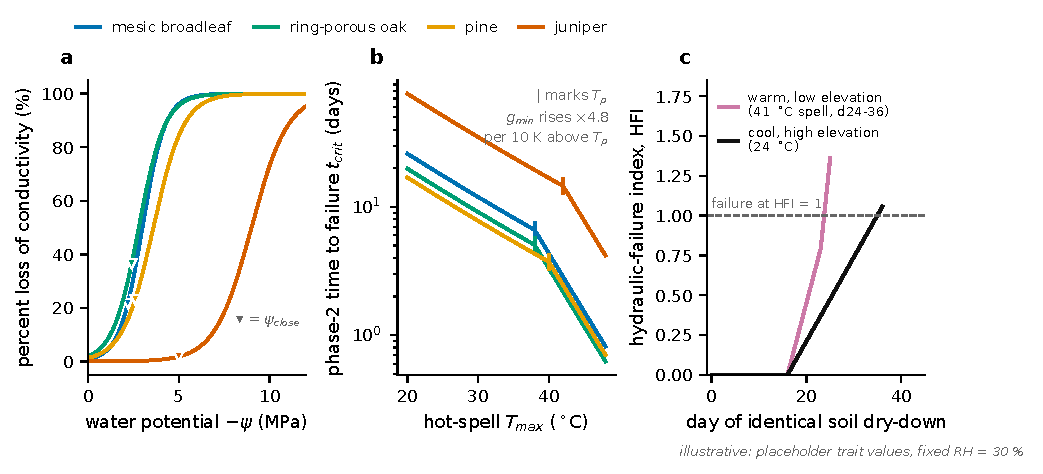
\includegraphics[width=\linewidth]{fig3_hydraulics.pdf}
\caption{The hydraulic engine, with illustrative placeholder traits for four functional groups. (a)~Vulnerability curves; triangles mark the stomatal-closure potential. (b)~Phase-2 time to failure against hot-spell temperature at fixed relative humidity; $g_{\min}$ steepens the fall above each group's $T_p$ (tick). (c)~The same soil dry-down at a warm low site with a 41\,$^\circ$C spell and at a cool high site: closure occurs on the same day, failure much earlier at the warm site.}\label{fig:hyd}
\end{figure}

\subsection{From traits to a probability}
Trait values differ among individuals and are uncertain to us; the two must not be mixed. We therefore sample in two levels. An outer loop of 50 draws takes hyper-parameters (group means and spreads of $P_{50}$, $S$, $\psi_{\text{close}}$, $C$, $g_{25}$, $T_p$) from posteriors built on XFT, TRY and the $g_{\min}$ compilation and updated with local measurements; an inner loop of 200 draws samples individuals. The mechanistic annual hazard is the share of individuals that fail,
\begin{equation}\label{eq:hmech}
\hmech_{iky}=\frac1M\sum_{m=1}^{M}\ind\Big[\max_{d\in y}\HFI^{(m)}_{iky,d}\ge1\Big],
\end{equation}
and the spread of $\hmech$ across the outer loop is its knowledge uncertainty. Seedlings, established saplings and mature trees form separate trait classes because capacitance per unit leaf area, rooting depth and $\psi_{\text{close}}$ change with ontogeny, and because larger trees are more exposed to drought \citep{Bennett2015}.

\textbf{Emulation.} Running the engine for every 30~m cell, year and draw is not feasible, so we emulate it. A Latin hypercube over stress-spell summaries (longest closed spell, mean $\VPD_{24}$ and $T$ during it, number of closed days) and trait-group descriptors is passed through the full engine, and a gradient-boosting regressor with monotone constraints (increasing in spell length, VPD and temperature; decreasing in $C$ and $B$) is fitted to $\hmech$. Monotonicity is guaranteed by construction, and the emulator must reproduce the full engine on a held-out hypercube to within 0.02 in absolute hazard before it is used.

\subsection{Pattern-oriented calibration, and what Module B does not claim}\label{sec:pom}
Prior trait draws are constrained by the patterns that Armenia already exhibits, using approximate Bayesian computation \citep{Grimm2005,Beaumont2010}. A draw $\theta$ is run over 2000--2024 forcing at reference sites and accepted if its summary statistics fall within a tolerance of the observed ones: (i) the Boyce index of predicted viability against present-day adult occurrence for each group; (ii) rank correlation between engine-predicted failure years and tree-ring growth collapses at the chronology sites \citep{Voss2025,Stepanyan2026,OpalaOwczarek2021}; (iii) observed dieback frequency by elevation band; and (iv) published orderings from dry-down experiments \citep{Waite2026}. The posterior narrows the priors; whatever mismatch remains is absorbed by a two-parameter recalibration on the link scale, $\cloglog(\tilde h^{\text{mech}})=a_g+b_g\,\cloglog(\hmech)$ with $b_g>0$, fitted per functional group on the observed event panel with hierarchical shrinkage. A monotone map of the link cannot change the shape of the physical response, so extrapolation keeps its mechanistic form.

The engine assumes constant capacitance, a plant hydraulically isolated from the soil once stomata close, no explicit carbon-starvation pathway, leaf temperature equal to $T_{\max}$ (tested against a leaf--air offset), and a single hydraulic threshold per group. Each is a documented limitation and a sensitivity experiment; none is hidden in the code.

\section{Module C: a hazard model fitted to observed mortality}\label{sec:C}

Module B says what should happen to a tree of a given type. Module C says what has happened to the forests of Armenia, and it is the only part of the framework that is calibrated against outcomes. It is a discrete-time survival model on a panel of pixel-years.

\subsection{Response and population at risk}
The population at risk is every 30~m pixel that was forest at the start of the record, followed until a dieback event, until censoring by harvest or fire (which are competing events, handled in \S\ref{sec:E}), or until the end of 2024. This removes the survivorship bias of v1: pixels that died stay in the data as events. A dieback event in year $t$ is a standardised anomaly of annual maximum kNDVI, relative to the pixel's trailing 10-year median, below $-2$ that has not recovered above $-1$ within two seasons and coincides with no disturbance flag; the segmentation algorithm (LandTrendr or CCDC; \citealt{Kennedy2010,Zhu2014}) and thresholds are fixed in the configuration and versioned. Because satellite dieback is an imperfect measure of mortality, sensitivity $\mathrm{Se}$ and specificity $\mathrm{Sp}$ are estimated on a stratified sample of interpreted pixel-years, and the observed hazard is corrected with the standard misclassification identity \citep{Rogan1978},
\begin{equation}\label{eq:rogan}
h_{\text{obs}}=\mathrm{Se}\,h+(1-\mathrm{Sp})(1-h)\quad\Longrightarrow\quad h=\frac{h_{\text{obs}}-(1-\mathrm{Sp})}{\mathrm{Se}+\mathrm{Sp}-1},
\end{equation}
or the same relation is embedded in the likelihood. Tree-ring growth collapses (ring width below 40\,\% of the trailing 10-year median) form a second, independent response on the chronology network; they are used to test temporal skill and to link the remote-sensing definition to physiological stress.

\subsection{The model}
Let $h_{i,t}=\Prob(T_i=t\mid T_i\ge t,\,\text{history})$ be the annual hazard of pixel $i$. We use the complementary log-log link, the discrete-time counterpart of proportional hazards \citep{Prentice1978,Singer2003}:
\begin{equation}\label{eq:cloglog}
\cloglog(h_{i,t})=\ln\!\big[-\ln(1-h_{i,t})\big]=\ln\Delta_{i,t}+\eta_{i,t},\qquad S_i(t)=\prod_{s\le t}(1-h_{i,s})=\exp\!\Big(-\sum_{s\le t}\Delta_{i,s}\,e^{\eta_{i,s}}\Big),
\end{equation}
where the offset $\ln\Delta$ lets periods of unequal length (censoring within a year) enter one likelihood, and the identity on the right is exact. The linear predictor is
\begin{equation}\label{eq:eta}
\eta_{i,t}=\beta_0+f(a_{i,t})+{\bm\beta_W}^{\!\top}\tilde{\bm x}_{i,t}+{\bm\beta_B}^{\!\top}\bar{\bm x}_i+\sum_{j=1}^{J}\sum_{k=1}^{K}\theta_{jk}\sum_{\ell=0}^{L}b_j(z_{i,t-\ell})\,c_k(\ell)+\bm\gamma^{\top}\bm u_{i,t}.
\end{equation}
Its parts have distinct jobs.

\textbf{Within and between (Mundlak).} Each climate covariate is split into a place mean and a departure, $\bar x_{i}=T_i^{-1}\sum_t x_{i,t}$ and $\tilde x_{i,t}=x_{i,t}-\bar x_i$ \citep{Mundlak1978,Bell2015}. $\bm\beta_W$ is the response to year-to-year departures at a fixed place, identified from within-place variation and therefore robust to any unmeasured, time-invariant site quality; it is the closest thing in the data to the effect of weather on mortality. $\bm\beta_B$ describes differences between places and contains adaptation, stand structure and everything else that differs across sites. Confounding of the two is how space-for-time substitution goes wrong, so the model keeps them apart.

\textbf{Drought legacies.} The cross-basis term is a distributed-lag non-linear model \citep{Gasparrini2010}: the exposure $z$ (water-stress integral or CWD anomaly) enters through a spline basis $b_j$ and its effect is spread over lags $\ell=0,\dots,L$ ($L=4$~yr) through a second basis $c_k$. Drought legacies of several years are pervasive in forests \citep{Anderegg2015}, and a model without lags mistakes them for noise.

\textbf{Stand terms.} $a_{i,t}$ is time since disturbance or planting, and $\bm u_{i,t}$ contains canopy height class, species-group composition and stand density proxies, with a size$\times$stress interaction whose sign is constrained a priori \citep{Bennett2015}. Coordinates and raw elevation are excluded: anything geographic must reach the model through a physical driver, or it is a place label that cannot be projected.

\textbf{Rare events.} All events are kept; non-events are sampled within blocks with known fraction $\pi_0$ and weighted by $1/\pi_0$, which gives a consistent estimator of the full-data model \citep{King2001}. Uncertainty comes from a block bootstrap, not from the pixel-level standard errors, which are meaningless under spatial dependence.

\subsection{Learners, stacking and the gate}\label{sec:gate}
Three learners share the panel: (i) an elastic-net cloglog GLM, transparent and extrapolating linearly on the link scale, which is at least an assumption one can read; (ii) gradient boosting with monotone constraints on physically signed covariates (hazard non-decreasing in CWD, VPD, heat and stress duration; non-increasing in plant-available water); and (iii) as a benchmark only, a random forest, which cannot extrapolate. Out-of-fold link-scale predictions of (i) and (ii) are combined by non-negative least squares with weights summing to one \citep{Wolpert1992,Breiman1996}, inside a nested cross-validation so that stacking weights are never fitted on the data they are scored on. The result, $\hstat$, is trustworthy only where the data are.

To decide where, we compute the dissimilarity index of \citet{Meyer2021}: the distance from a prediction cell to its nearest training cell in a standardised, importance-weighted covariate space, divided by the mean pairwise training distance, $\DI(x)=\min_j\|x-x_j\|/\bar d$. The threshold $\DI^\ast$ is the upper whisker of the training cells' own $\DI$ values, each computed against training cells in \emph{other} cross-validation folds, so that it reflects the distances over which the model was actually validated. The final hazard blends on the link scale,
\begin{equation}\label{eq:gate}
\begin{aligned}
\cloglog(h)&=w\,\cloglog(\hstat)+(1-w)\,\cloglog(\tilde h^{\text{mech}}),\\
w&=\exp\!\big[-\kappa\,\max\{0,\,\DI/\DI^\ast-1\}\big],\qquad\kappa=2,
\end{aligned}
\end{equation}
so that $w=1$ inside the area of applicability, decays smoothly outside it, and cumulative hazards, not probabilities, are what get mixed. The share of cells and years outside the area of applicability is reported as an output for every scenario, the \emph{extrapolation footprint}: a statement of how much of the projected future rests on physics rather than on observation.

\subsection{Bounding the space-for-time assumption}
Projecting the within and between effects requires a decision about whether trees adapt to the shifted mean. We do not make it; we bracket it. With $x^{\text{proj}}_{i,t}$ the projected covariate and $\bar x^{\text{hist}}_i$, $\bar x^{\text{proj}}_i$ the historical and projected 20-year place means,
\begin{equation}\label{eq:bracket}
\eta^{\text{no adapt}}_{i,t}:\ \ \tilde x=x^{\text{proj}}_{i,t}-\bar x^{\text{hist}}_i,\ \ \bar x=\bar x^{\text{hist}}_i;\qquad
\eta^{\text{full acclim}}_{i,t}:\ \ \tilde x=x^{\text{proj}}_{i,t}-\bar x^{\text{proj}}_i,\ \ \bar x=\bar x^{\text{proj}}_i.
\end{equation}
In the first, the within-place response applies to the whole climatic shift; in the second, $\bm\beta_B$, typically weaker because trees are adapted to their local mean, applies to the shift of the mean. Every projection is reported as this bracket, and the width between the bounds is itself a result: it measures how much of the future depends on an ecological assumption that no dataset can currently settle.

\section{Modules D and E: forest ecology, growth and cohort viability}\label{sec:DE}

\subsection{Module D: niche, attainable height, growth and establishment}\label{sec:D}
\textbf{Adult niche as a consistency test.} For each species we fit a penalised presence--background model on physically meaningful predictors (CWD, growing degree days, winter minimum, VPD, soil), with the background drawn from a target-group sample to absorb collection bias, and score it under spatial-block CV with the continuous Boyce index \citep{Hirzel2006}. With $P/E_b=(n^{\text{pres}}_b/n^{\text{pres}})/(n^{\text{bg}}_b/n^{\text{bg}})$ in suitability bin $b$, $\mathrm{CBI}=\rho_s(b,\,P/E_b)$, the Spearman rank correlation across bins, which needs no presence--absence data and no threshold. The niche is deliberately not a driver of $V$. It is a realised niche, shaped by competition, dispersal and land use; in the Caucasus competition alone contracts fundamental niche areas by a factor of 1.2--1.7 \citep{Pshegusov2022}, so it would veto exactly the sites where planting is most useful. Its job is consistency: sites with high $V$ should be enriched among adult occurrences, and the mismatch map separates climatic limitation from dispersal or land-use limitation.

\textbf{Attainable height.} Observed canopy height reflects age and disturbance history as much as site quality, so its mean is a poor measure of potential. We estimate the upper envelope, as in site-index work \citep{Skovsgaard2008}, by quantile regression \citep{Cade2003} of GEDI and canopy-height-model heights on climate, soil and terrain,
\begin{equation}\label{eq:qr}
H^\ast(x)=\hat f_\tau(x),\qquad \hat f_\tau=\arg\min_f\sum_i\rho_\tau\big(H_i-f(x_i)\big),\quad \rho_\tau(u)=u\,\big(\tau-\ind[u<0]\big),\quad\tau=0.9,
\end{equation}
scored by pinball loss and by coverage of the $\tau$-quantile on held-out blocks, with conformalised quantile regression intervals \citep{Romano2019}. Outside the area of applicability, $H^\ast$ falls back on a water-limited scaling by the transpiration ratio $\mathrm{AET}/\mathrm{PET}$ from Module~A.

\textbf{Growth in physiological age.} Height follows the Chapman--Richards curve in a physiological age that advances more slowly in stress years,
\begin{equation}\label{eq:cr}
H(a)=H^\ast\,\big(1-e^{-k a}\big)^{p},\qquad a_{y+1}=a_y+\varphi_y,\qquad \varphi_y=f_W\,f_T\,f_F,\qquad f_W=\frac{1}{1+(\CWD_y/\CWD_{50})^{m}},
\end{equation}
where $f_T$ is a growing-degree-day modifier, $f_F$ a late-frost modifier, $\varphi_y\in(0,1]$ (Liebig-type limitation as in 3-PG; \citealt{Landsberg1997}) and $\CWD_{50}$, $m$ are estimated from the tree-ring growth--CWD relation. Stress years delay development without reversing it, which keeps the closed form. The age at which a cohort reaches $\Hmin$ is $a^\ast=-k^{-1}\ln\!\big[1-(\Hmin/H^\ast)^{1/p}\big]$ (infinite if $\Hmin\ge H^\ast$), and $\Prob[H_T\ge\Hmin]=\Prob[\sum_{y\le T}\varphi_y\ge a^\ast]$ is evaluated over ensemble members and parameter draws. This is also where Module~A gets its leaf area: LAI follows $H(a)$, closing the loop between stand development and stand water use.

\textbf{Establishment.} The regeneration niche is narrower than the adult niche \citep{Jackson2009,Dobrowski2015,Davis2019}, and the pattern is visible locally: the southern beech stand shows mature trees and no regeneration \citep{Stepanyan2026}. Planted seedlings pass through the same bottleneck, with shallow roots and little storage. Establishment is therefore a discrete-time hazard over the years until height exceeds a vulnerability height $H_{\text{est}}$,
\begin{equation}\label{eq:est}
h^{\text{est}}_{\tau}=\cloglog^{-1}\!\big(\beta_0+\bm\beta^{\top}\bm x_\tau+g(\tau)\big),\qquad S_{\text{est}}=\prod_{\tau}\big(1-h^{\text{est}}_\tau\big),
\end{equation}
with covariates in the first seasons after planting: minimum topsoil $\REW$, peak $\VPD_{\text{day}}$, heat days, late frosts, snow-cover duration, stock type and size, browsing protection and planting method. Data are plantation follow-up surveys and regeneration plots. The window length $\tau\le\tau_{\max}$ is set by the growth module, so that a site that slows growth also prolongs exposure.

\subsection{Module E: cohort viability, refugia and analogues}\label{sec:E}
\textbf{Competing hazards.} The all-cause annual hazard combines the mechanism-specific hazards $h_{k,y}$ for establishment, hydraulic failure, late frost, fire and biotic agents,
\begin{equation}\label{eq:htot}
h^{\mathrm{tot}}_{y}=1-\prod_k\big(1-h_{k,y}\big),\qquad V=\Big[\prod_{y=1}^{T}(1-h^{\mathrm{tot}}_y)\Big]\cdot\Prob[H_T\ge\Hmin],
\end{equation}
which is Eq.~\eqref{eq:V} with its factors named. $h_{\text{hyd}}$ is the gated hazard of Eq.~\eqref{eq:gate}; $h_{\text{frost}}$ and $h_{\text{fire}}$ are cloglog models on the late-frost index and on a fire-weather index with burned-area records; $h_{\text{bio}}$ (insects, disease, browsing) is a baseline from long-term plot mortality and is not projected with climate, which we state as a limitation rather than pretend otherwise. The product assumes independence conditional on covariates; it is tested by comparing the modelled all-cause hazard with observed all-cause plantation mortality, and compound events such as drought followed by fire enter as interactions in Module C.

\textbf{Robust refugia.} A cell is a refugium for option $k$ at horizon $T$ only if it is viable in most of the ensemble, topographically decoupled from regional exposure, and inside the area of applicability:
\begin{equation}\label{eq:refug}
R_{ik}=\ind\big[\Prob_\omega(V_{ik}\ge v^\ast)\ge\rho\big]\cdot\ind[B_i>0]\cdot\ind[\DI\le\DI^\ast],\qquad B_i=\frac{\bar E_{\text{reg},i}-E_i}{\mathrm{sd}(E)},
\end{equation}
with $v^\ast=0.6$, $\rho=0.8$ as defaults, $E$ a standardised composite of CWD, growing-season VPD and heat exposure, and $\bar E_{\text{reg},i}$ its mean within a regional radius. Cells outside the area of applicability are flagged, not asserted. A risk-averse continuous score, $\mathrm{median}(V)-\lambda\,\mathrm{IQR}(V)$ across the ensemble, ranks cells within the refugium class.

\textbf{Climate analogues.} For each cell and future window we find the present-day cell with the closest climate, using Mahalanobis distance in standardised space (mean and winter-minimum temperature, CWD, VPD, GDD, precipitation seasonality) under the covariance of the reference climate, and the novelty percentile of the distance among reference nearest-neighbour distances \citep{Mahony2017}. Two uses follow. Existing stands at the analogue location are candidate seed sources and provenance tests, with the usual caveat about local adaptation; and no-analogue cells are flagged as places where no statistical or niche model, ours included, should be trusted, which complements the area of applicability with a purely climatic criterion.

\section{The machine-learning pipeline and how it is validated}\label{sec:ml}

The v1 pipeline failed at evaluation, not at fitting. A random split of spatially autocorrelated pixels rewards a model for memorising place, and the score it produced described a task (interpolating inside the same landscape and era) that nobody needs done. Version 2 follows one rule: a headline number is computed under the resampling design that mimics the use it will be put to, against baselines that could embarrass the model, and every fitted quantity, meaning hyper-parameters, feature choices, stacking weights, the applicability threshold and the recalibration constants of Module~B, is fitted inside the training fold only.

\subsection{Three kinds of transfer, six designs}
The framework is used to predict in places it has not seen, in years it has not seen and in climates it has not seen. These are different tasks and no single split covers them; Table~\ref{tab:cv} lists the designs, and the pass criteria are written down now, before any model is fitted. They are defaults to be confirmed at the first gate (\S\ref{sec:plan}), not thresholds tuned to a result.

\begin{table}[t]
\centering
\caption{Validation designs. BSS is the Brier skill score against the stated baseline; the criteria are pre-specified defaults.}\label{tab:cv}
\footnotesize
\begin{tabularx}{\linewidth}{@{}>{\raggedright\arraybackslash\bfseries\sffamily}p{2.55cm}>{\raggedright\arraybackslash}p{4.3cm}>{\raggedright\arraybackslash}p{3.2cm}>{\raggedright\arraybackslash}X@{}}
\toprule
Design & What is held out & Question it answers & Pre-specified criterion\\
\midrule
Spatial-block CV (5 folds, repeated) & Blocks with side $\ge$ residual-variogram range (25~km until estimated), 2~km buffer, folds balanced by event count & New places, same period & BSS vs.\ coordinates-only $\ge0.10$; calibration slope 0.8--1.2\\
Forward chaining & All pixels in years $t{+}1..t{+}3$ after training on years $\le t$ (at least 10 training years) & New years & BSS vs.\ persistence $>0$ at every origin\\
Leave-province-out & One administrative province at a time & Transfer to a management region & BSS $>0$ in the worst province\\
Leave-extreme-year-out & The $k$ driest or hottest years by national SPEI-12 & The years that matter most & Observed event count inside the 90\,\% bootstrap band of predicted\\
Extrapolation CV & Hottest and driest 30\,\% of cells on a CWD--$T_{\max}$ composite; train on the rest & Warmer, drier than seen & Gated hybrid log-loss $\le$ best single component; $\rho_s(\DI,\text{error})\ge0.4$\\
Design-based sample & Independent probability sample of plots (\S\ref{sec:design-based}) & Is the map right, with an honest interval? & Predicted vs.\ observed per class within $\pm0.10$\\
\bottomrule
\end{tabularx}
\end{table}

\textbf{Blocks.} The block side is the practical range of the empirical variogram of residuals from a climate-only model, the distance beyond which residuals are effectively independent \citep{Roberts2017,Valavi2019}. It is then checked with nearest-neighbour distance matching \citep{Mila2022}, which compares the distribution of distances from test to training points in the cross-validation with that from prediction locations to training locations; if the cross-validation is easier than the real task, the blocks are enlarged. Ploton and colleagues showed how badly a random split can overstate large-scale ecological mapping skill \citep{Ploton2020}, and v1's coordinates-only benchmark (Table~\ref{tab:audit}) is the same lesson at small scale. \citet{Meyer2022} add that a map's accuracy statement should travel with the domain in which it was validated, which in this framework is the role of the area of applicability.

\textbf{Nesting.} All tuning runs in an inner loop confined to the outer training blocks. The applicability threshold $\DI^\ast$, the stacking weights and the link-scale recalibration $(a_g,b_g)$ of Module~B are treated as model parameters and are refitted in every outer fold, so that no outer test cell has ever influenced them.

\subsection{Baselines and metrics}
Every design is scored against four baselines: a climatological null (each year's base rate), persistence (the pixel's own event history), a coordinates-only model (a smooth spatial function of position and nothing else) and a replica of the v1 random forest. The coordinates-only benchmark matters most. In the v1 data it explained more variance than the climate deltas did (Table~\ref{tab:audit}); a model that cannot beat a map of its own coordinates has learnt \emph{where}, not \emph{why}.

The hazard model is probabilistic, so it is scored with proper scoring rules. For $N$ person-periods with outcomes $y_j\in\{0,1\}$ and predicted hazards $\hat p_j$, weighted by $1/\pi_0$ for sampled non-events,
\begin{equation}\label{eq:brier}
\mathrm{BS}=\frac1N\sum_{j}(\hat p_j-y_j)^2,\qquad \mathrm{BSS}=1-\frac{\mathrm{BS}}{\mathrm{BS}_{\text{ref}}},\qquad
\mathrm{BS}=\underbrace{\tfrac1N\sum_b n_b(\bar p_b-\bar o_b)^2}_{\text{reliability}}-\underbrace{\tfrac1N\sum_b n_b(\bar o_b-\bar o)^2}_{\text{resolution}}+\underbrace{\bar o(1-\bar o)}_{\text{uncertainty}},
\end{equation}
with the second identity the Murphy decomposition over probability bins $b$. Reliability is the part that matters for decisions, because a hazard that is systematically too high or low changes the ranking of options once it is compounded over 30 years. Calibration is also tested directly by regressing the outcome on the logit of the prediction, $\operatorname{logit}\Prob(y=1\mid\hat p)=a+b\,\operatorname{logit}\hat p$, for which the target is $a=0$, $b=1$; a slope below 1 signals over-fitting, above 1 under-confidence \citep{Steyerberg2010}. The log-loss is the discrete-time likelihood and doubles as the fitting criterion. Because dieback is rare, precision--recall AUC is reported; ROC AUC is reported but never as a headline, since it ignores both calibration and base rate. Expected calibration error is a summary with a known dependence on binning and is never used alone; cumulative-hazard calibration (predicted against observed cumulative incidence by risk decile) is the check that matches the $30$-year use. Overall accuracy and Cohen's $\kappa$ are not used \citep{Pontius2011}. Continuous outputs (attainable height) are scored by the pinball loss of Eq.~\eqref{eq:qr} and by empirical coverage.

\subsection{Prediction intervals, and where they stop being valid}
For attainable height we wrap the quantile models in conformalised quantile regression \citep{Romano2019}: with lower and upper quantile fits $\hat q_{lo},\hat q_{hi}$ and calibration scores $E_i=\max\{\hat q_{lo}(x_i)-y_i,\ y_i-\hat q_{hi}(x_i)\}$, the interval $[\hat q_{lo}(x)-\hat Q,\ \hat q_{hi}(x)+\hat Q]$ with $\hat Q$ the $\lceil(1-\alpha)(n+1)\rceil/n$ empirical quantile of $E_i$ has marginal coverage $\ge1-\alpha$ under exchangeability \citep{Angelopoulos2023}. Under covariate shift the scores can be re-weighted by the density ratio between target and calibration covariates \citep{Tibshirani2019}, but the ratio is undefined where the calibration data have no mass. That is precisely the extrapolation regime, so we do not claim coverage there; intervals outside the area of applicability are drawn hatched, and their empirical coverage is measured in the extrapolation CV and reported.

Applicability is validated as well as used. If the dissimilarity index is informative, prediction error should grow with it; we report skill stratified by $\DI/\DI^\ast$ in the extrapolation CV, and the gate of Eq.~\eqref{eq:gate} is admissible only if the rank correlation between $\DI$ and absolute error is at least 0.4. The decay constant $\kappa=2$ is a default checked against $\kappa\in\{1,2,4\}$ on the same held-out tail.

\subsection{Why in-range validation cannot rank extrapolators: a controlled experiment}
Everything above measures skill on data that resemble the training data. The limits of that are easiest to see in a world where the truth is known. We built two synthetic worlds from the engine of Module~B in which mortality hazard depends on hot-spell temperature and a soil-water index. Training data cover $T_{\max}=24$--34\,$^\circ$C only. The worlds differ in a single trait, the temperature $T_p$ at which residual conductance steepens (38\,$^\circ$C in world A, 47\,$^\circ$C in B), so the data inside the training range are practically indistinguishable, while the hazard beyond it is not (Fig.~\ref{fig:extrap}a,b). Four learners are fitted to the same data: a random forest, the cloglog GLM, the mechanistic model alone (deliberately mis-specified by $+2$\,$^\circ$C in $T_p$, with wider trait spreads and 15\,\% higher capacitance) and the AOA-gated hybrid.

\begin{figure}[t]
\centering
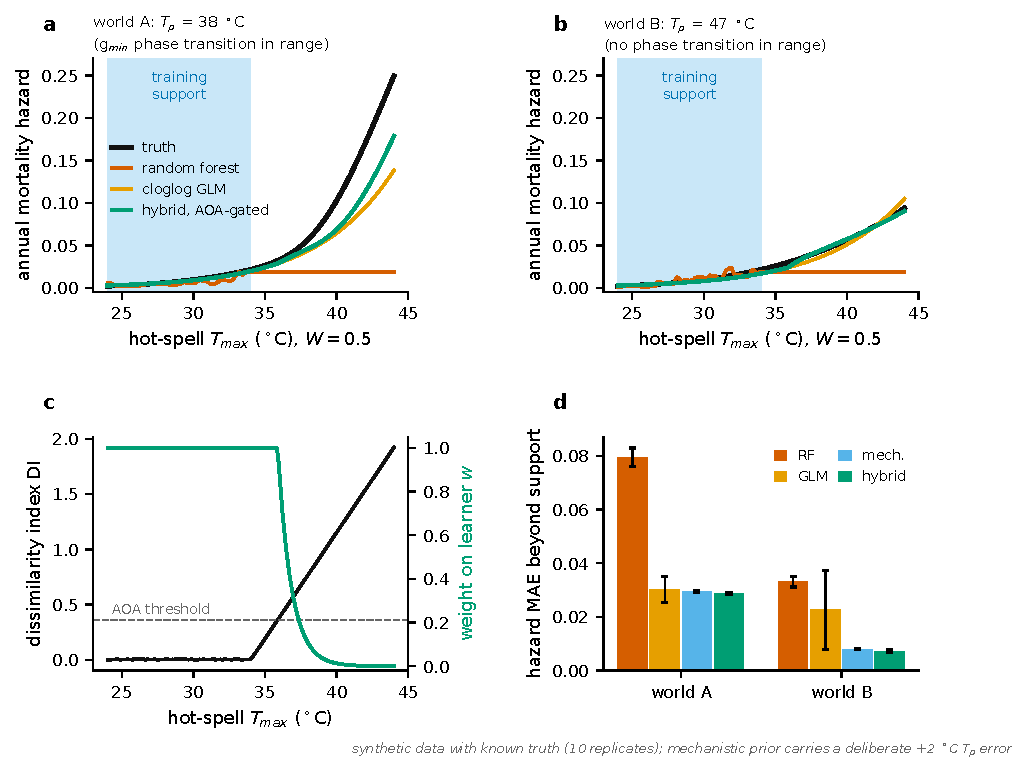
\includegraphics[width=\linewidth]{fig4_extrapolation.pdf}
\caption{Controlled extrapolation experiment on synthetic data with known truth (10 replicates). (a,b)~True hazard and model predictions at fixed soil-water index; the shaded band is the training support. (c)~Dissimilarity index and gate weight $w$ along the temperature axis; the gate hands over to the mechanistic model as the index passes its threshold. (d)~Mean absolute hazard error beyond the training support (mean $\pm$ s.d. of replicates). Illustrative: it demonstrates a mechanism, not the size of the effect in Armenia.}\label{fig:extrap}
\end{figure}

Inside the training range all four methods err by 0.001--0.003 in absolute hazard and cannot be ranked. Beyond it the mean absolute error is, for world A (true mean hazard 0.101), 0.080 for the random forest, 0.030 for the GLM, 0.029 for the mechanistic model and 0.029 for the hybrid; for world B (true mean 0.054), 0.033, 0.023, 0.008 and 0.007. The random forest is worst in both because it holds its last in-range value, as v1's did. The GLM's linear extrapolation on the link scale is an assumption: in B it follows the truth in the typical replicate but its error varies widely (standard deviation 0.015 across replicates), and in A it misses the phase transition. The mechanistic and hybrid models have the lowest error in both worlds, in A only marginally below the GLM, and the hybrid cures nothing: in world A it still under-predicts because its prior places $T_p$ too high, so the transition arrives late. What the design achieves is narrower, and we think more defensible. Extrapolation is made by a model whose form is physically motivated rather than by an accident of the learner; the switch to it is governed by a documented, testable criterion (Fig.~\ref{fig:extrap}c); and its remaining error is bounded by the error of the mechanistic prior, which Module~B's calibration and sensitivity experiments are built to expose.

\subsection{Independent, design-based validation of the products}\label{sec:design-based}
Cross-validation estimates how a modelling procedure performs on new data; it does not estimate the accuracy of the final map, and with clustered or purposive reference data it can mislead in either direction \citep{Wadoux2021}. The claims that will be made to foresters and funders are claims about maps, so they are backed by an independent probability sample whose inference needs no model of spatial structure \citep{Olofsson2014,Stehman2019}. Strata $h$ are cross-classifications of predicted-$V$ class, area-of-applicability status and elevation zone, with stratum weights $W_h$ from mapped areas. The stratified estimator of a proportion (a dieback frequency, or a survival-and-height frequency) and its variance are
\begin{equation}\label{eq:strat}
\hat p=\sum_h W_h\,\bar y_h,\qquad \widehat{\mathrm{Var}}(\hat p)=\sum_h W_h^2\,\frac{s_h^2}{n_h},\qquad n\approx\Big(\frac{\sum_h W_h S_h}{S(\hat p)}\Big)^{2},\quad S_h=\sqrt{p_h(1-p_h)},
\end{equation}
where $S(\hat p)$ is the target standard error and the last expression is the sample size for that target given anticipated stratum proportions $p_h$. For four strata with $W=(0.4,0.3,0.2,0.1)$ and $p=(0.05,0.20,0.50,0.80)$, $\sum_hW_hS_h=0.347$, and a standard error of 0.02 requires $n\approx300$ plots, against about 480 under simple random sampling; this is the origin of the 300-plot minimum in \S\ref{sec:data}. Allocation is proportional to $W_hS_h$ with a floor of 25 plots per stratum and deliberate over-sampling of strata outside the area of applicability. The plots are fixed before any model is fitted, are excluded from training together with a buffer, and accuracy is reported separately inside and outside the area of applicability.

There is one thing no design can do: validate a projection against observations that do not yet exist. What is validated is the machinery that produces projections, in hindcast, in transfer and in extrapolation, and every projected map is accordingly published with its extrapolation footprint instead of an accuracy figure it cannot have.

\section{Scenarios, uncertainty and the decision layer}\label{sec:unc}

\subsection{Scenario and ensemble design}
Scenarios are choices about the world, not draws from a distribution, and we do not average them. Results are reported per pathway (SSP1-2.6, SSP2-4.5, SSP3-7.0, SSP5-8.5), with SSP5-8.5 used as a high-end stress test rather than a forecast \citep{Hausfather2020}, at 20-year windows centred on 2050, 2080 and 2100 against the fixed 1991--2020 reference. The primary ensemble is the five ISIMIP3b models; NEX-GDDP-CMIP6 supplies SSP2-4.5 and a wider model set to test whether conclusions depend on that particular five.

Two safeguards address the fact that CMIP6 contains models whose sensitivity exceeds the assessed likely range. Every headline result is indexed by global warming level (1.5, 2, 3 and 4~K above pre-industrial) as well as by calendar year, which removes model sensitivity from the argument about \emph{when}; and ensemble statistics are shown with and without any model above the assessed very-likely upper bound of equilibrium sensitivity \citep{Hausfather2022,Zelinka2020}. Performance--independence weighting \citep{Brunner2020} is a sensitivity analysis, never the default. Where overshoot runs exist (SSP5-3.4-OS), they serve as a stress test of the lag structure of Module~C: if a cohort's viability at 2100 differs between a warming-then-cooling path and a monotone path that ends at the same climate, the framework is representing legacy and hysteresis, the trajectory dependence reported for Amazon dieback under overshoot \citep{Munday2025}.

\subsection{Partitioning uncertainty}
The output $V$ is itself a probability, so the ensemble yields a distribution over probabilities. Its spread has different origins that call for different responses (Table~\ref{tab:unc}), and the framework reports them separately: a scientist can reduce knowledge uncertainty by measuring, a manager can reduce exposure to scenario uncertainty by diversifying, and neither can do anything about internal variability except plan for it.

\begin{table}[t]
\centering
\caption{Factors of the uncertainty ensemble.}\label{tab:unc}
\footnotesize
\begin{tabularx}{\linewidth}{@{}>{\raggedright\arraybackslash\bfseries\sffamily}p{3.0cm}>{\raggedright\arraybackslash}p{4.4cm}>{\raggedright\arraybackslash}p{3.0cm}>{\raggedright\arraybackslash}X@{}}
\toprule
Factor & Levels & Kind & Treatment\\
\midrule
Pathway (SSP) & 4, plus overshoot stress test & Deep (a choice) & Conditional reporting; never averaged\\
Climate model & 5 (ISIMIP3b); wider set (NEX-GDDP) & Structural & GWL indexing; with/without hot models\\
Internal variability & Years within 20-yr windows, realisations & Aleatory & Distribution of annual hazards\\
Downscaling & QDM, delta change & Structural & Both carried\\
PET formulation & 4 (\S\ref{sec:A}) & Structural & All carried\\
Soil and rooting depth & 50 draws & Epistemic & Random draws from SoilGrids quantiles and priors\\
Traits & 50 hyper-parameter $\times$ 200 individual draws & Epistemic and aleatory & Two-level Monte Carlo (\S\ref{sec:B})\\
Model class & Statistical, mechanistic, gated hybrid & Structural & All reported; hybrid is the default product\\
\bottomrule
\end{tabularx}
\end{table}

\textbf{Analysis of variance for discrete factors.} For an output $Y$ (for example regional mean $V$ or the area with $V\ge v^\ast$) evaluated on the crossed design of the discrete factors, the total variance is split by a standard ANOVA into main effects and interactions, $\mathrm{Var}(Y)=\sum_f \mathrm{Var}_f+\text{interactions}$, and the fractions $F_f=\mathrm{Var}_f/\mathrm{Var}(Y)$ are tracked as a function of lead time in the manner of \citet{Hawkins2009} and \citet{Lehner2020}. This tells us, for each horizon and region, whether the argument is about emissions, about the climate model, or about our own modelling.

\textbf{Global sensitivity for the knowledge factors.} For the continuous, epistemic factors $X=(X_1,\dots,X_k)$ (rooting depth, plant-available water, trait hyper-parameters, recalibration constants) we use variance-based indices computed on the emulator of Module~B, since the full engine is too slow for the number of evaluations needed. The first-order and total-order indices are
\begin{equation}\label{eq:sobol}
S_i=\frac{\mathrm{Var}\big[\E(Y\mid X_i)\big]}{\mathrm{Var}(Y)},\qquad S_{T_i}=\frac{\E\big[\mathrm{Var}(Y\mid X_{\sim i})\big]}{\mathrm{Var}(Y)}\ \approx\ \frac{1}{2N\,\widehat{\mathrm{Var}}(Y)}\sum_{j=1}^{N}\Big[f(A)_j-f\big(A_B^{(i)}\big)_j\Big]^2,
\end{equation}
with the Jansen-type total-order estimator recommended by \citet{Saltelli2010}, in which $A$ and $B$ are independent sample matrices and $A_B^{(i)}$ is $A$ with column $i$ taken from $B$; the cost is $N(k+2)$ emulator runs. A large $S_{T_i}-S_i$ marks interactions, which in a threshold system like this one (phase transition, stomatal closure) are expected and should not be hidden. The result is a ranked list of which measurement would reduce uncertainty most, and it sets the priorities of the trait campaign in \S\ref{sec:plan}.

\subsection{Decision layer: robust portfolios}
Ranking species by expected viability cell by cell yields a landscape planted to whichever option is best on average, and that landscape fails all at once in the scenarios where the option is not. A planting programme is a portfolio, so it is optimised as one.

Let $u$ index management units (aggregated 30~m cells, roughly 1~ha), $j$ planting options, and $\omega\in\Omega$ the members of the scenario ensemble. Let $x_{uj}\in\{0,1\}$ indicate that option $j$ is planted in unit $u$, $A_u$ its area, and $b_{uj\omega}=V_{uj\omega}\,v_j$ the benefit per hectare, viability times a value weight $v_j$ (canopy area, carbon or water services, set with stakeholders). The benefit of a plan in scenario $\omega$ is $B_\omega(x)=\sum_{u,j}A_u\,b_{uj\omega}\,x_{uj}$. The plan maximises a mixture of the mean and the mean of the worst tail,
\begin{equation}\label{eq:cvar}
\max_{x,\zeta,s}\ \ (1-\lambda)\,\frac1{|\Omega|}\sum_\omega B_\omega(x)\;+\;\lambda\Big[\zeta-\frac{1}{(1-\alpha)|\Omega|}\sum_\omega s_\omega\Big]\quad\text{s.t.}\quad s_\omega\ge\zeta-B_\omega(x),\ \ s_\omega\ge0,
\end{equation}
where the bracket is the conditional value-at-risk, the mean benefit over the worst $(1-\alpha)$ share of scenarios, in the linear form of \citet{Rockafellar2000}. The remaining constraints are
\begin{equation}\label{eq:mip}
\sum_j x_{uj}\le1,\qquad \sum_{u,j}A_u\,c_{uj}\,x_{uj}\le\mathrm{Budget},\qquad \sum_uA_u x_{uj}\le\sigma_{\max}\sum_{u,j'}A_u x_{uj'},\qquad x_{uj}\le e_{uj},
\end{equation}
one option per unit, a budget, a cap $\sigma_{\max}$ on the area share of any single option (response diversity), and an eligibility indicator $e_{uj}$ that is zero where the option is outside its applicability region or legally excluded. A per-basin cap on additional water use can be added as a further linear constraint. The problem is a mixed-integer linear programme, solved with HiGHS in the skeleton. With about 500 scenario members, $\alpha=0.8$ (the worst 100), a few thousand units and ten to fifteen options, it has of the order of $10^4$--$10^5$ binary variables, which is tractable after aggregation and, if necessary, scenario reduction.

Sweeping $\lambda$ from 0 to 1 traces the mean--CVaR frontier, and the distance between its ends is the price of robustness, expressed in units of benefit (hectares of expected surviving canopy for canopy-area weights). The optimiser exploits whatever its scenario sample happens to contain, so the reported CVaR is evaluated on a fresh, independent set of ensemble members; a large gap between the in-sample and out-of-sample values is a warning that the portfolio is over-fitted to the ensemble. Areas with a large extrapolation footprint are not silently planted or silently excluded: they are flagged, and the plan states how much of its expected benefit comes from cells outside the area of applicability.

\section{Work plan, gates, outputs and what would prove us wrong}\label{sec:plan}

\subsection{Work packages and go/no-go gates}
The plan is indicative and expressed in months from project start (24 in total); the calendar follows the funding decision. It is ordered so that the cheapest and most decisive questions are answered first: whether the physical drivers are right (WP2), and whether observed mortality can be predicted better than by a map of coordinates (WP4). The expensive parts, the field survey and the full ensemble, start only after the gates that justify them.

\begin{table}[t]
\centering
\caption{Work packages. Months are from project start.}\label{tab:wp}
\footnotesize
\begin{tabularx}{\linewidth}{@{}>{\raggedright\arraybackslash\bfseries\sffamily}p{4.1cm}>{\raggedright\arraybackslash}p{1.4cm}>{\raggedright\arraybackslash}X@{}}
\toprule
Work package & Months & Main outputs\\
\midrule
WP1 Data, labels, harmonisation & 1--8 & Master grid and data manifests; versioned dieback panel; plot and ring database\\
WP2 Module A: topoclimate and water balance & 2--8 & 30~m forcing ensemble, PET ensemble, $\psi_s$; station cross-validation and closure tests\\
WP3 Traits and hydraulic engine & 3--14 & Trait posteriors; local $P_{50}$, $g_{\min}(T)$, pressure--volume curves for 4--6 species; emulator; ABC calibration\\
WP4 Mortality hazard model & 6--14 & Hazard stack, DI-based area of applicability, nested CV report\\
WP5 Growth, establishment, plantation survey & 4--18 & Attainable-height and growth models; establishment hazard; two field seasons of planting-follow-up plots\\
WP6 Uncertainty, viability and decision & 12--22 & Ensemble $V$, refugia, analogues; ANOVA and Sobol' partition; portfolio tool\\
WP7 Validation, products and dissemination & 1--24 & Design-based sample (months 14--20); model cards; papers; training for Armenian partners\\
\bottomrule
\end{tabularx}
\end{table}

Four gates decide whether the work continues as planned, and each names its fallback so that a failure is a result rather than a crisis.

\textbf{G1, month 8: physics and data are adequate.} Module A closes its water balance, its downscaled temperature and precipitation reduce the raw ERA5-Land error at held-out stations, and it reproduces TerraClimate CWD within a stated tolerance; the minimum data of \S\ref{sec:data} exist. \emph{Fallback:} coarsen to 100~m and extend the label network before fitting anything.

\textbf{G2, month 14: the hazard model earns its place.} Under spatial-block CV and forward chaining it meets the criteria of Table~\ref{tab:cv} against the coordinates-only and persistence baselines. \emph{Fallback:} the statistical component is retired to the role of benchmark, the mechanistic model is reported with widened uncertainty, and the failure itself, a negative result on dieback predictability from climate in this region, is published.

\textbf{G3, month 18: the gate is justified.} In the extrapolation CV the hybrid is no worse than the better of its components, $\rho_s(\DI,\text{error})\ge0.4$, and the emulator reproduces the full engine to within 0.02 in hazard. \emph{Fallback:} report mechanistic and statistical bounds separately instead of a blended hazard.

\textbf{G4, month 20: products are validated.} The design-based sample is complete and predicted $V$ agrees with observed class frequencies within $\pm0.10$, inside and outside the area of applicability separately. Maps and portfolios are released only after G4; before that they are labelled as provisional.

\subsection{Deliverables and publication plan}
The project produces an open-source package (the skeleton of \S\ref{sec:repo} developed to full implementation), versioned datasets of dieback labels and trait posteriors, viability, refugium and extrapolation-footprint layers with the uncertainty partition, a portfolio tool, a model card per product stating intended use, training data, validation results and known failure modes, and technical reports for the FORACCA partners. Three papers are planned; each stands on its own and none depends on the outcome of the others. Target venues are indicative and depend on the gate results.
\begin{enumerate}
\item \textbf{A hazard-model paper}: discrete-time cloglog survival modelling of forest dieback with within/between decomposition, drought legacies and label-error correction, for Armenia. Its central claim is methodological and testable: what the space-for-time assumption changes, measured by the width of the bracket in Eq.~\eqref{eq:bracket}. Candidate outlets: \emph{Global Change Biology}, \emph{Ecological Applications}.
\item \textbf{A methods paper}: gating a mechanistic and a statistical hazard model by area of applicability, with the controlled experiment of Fig.~\ref{fig:extrap} extended to real held-out climates. Candidate outlet: \emph{Methods in Ecology and Evolution}.
\item \textbf{A decision paper}: robust species--site portfolios under partitioned uncertainty, with the price of robustness and the value of measuring traits from the Sobol' analysis. Candidate outlets: \emph{Nature Sustainability}, \emph{Nature Communications}, or a specialist journal if the results warrant less.
\end{enumerate}

\subsection{Principal risks}
The six risks that most threaten the schedule or the claims are listed in Table~\ref{tab:risk} with their fallbacks; each is tied to a gate above, so that a problem surfaces at a decision point rather than in the final year.
\begin{table}[t]
\centering
\caption{Risk register (main items).}\label{tab:risk}
\footnotesize
\begin{tabularx}{\linewidth}{@{}>{\raggedright\arraybackslash\bfseries\sffamily}p{3.5cm}>{\raggedright\arraybackslash}p{4.7cm}>{\raggedright\arraybackslash}X@{}}
\toprule
Risk & Consequence & Mitigation and fallback\\
\midrule
Satellite dieback labels are too noisy & Biased hazards, weak signal & Misclassification correction (Eq.~\ref{eq:rogan}); tree-ring collapses as second response; interpret-and-verify sample\\
No local hydraulic traits for Caucasian species & Module B leans on priors & Hierarchical priors from XFT/TRY; measurement campaign for 4--6 species, targeted by the Sobol' ranking\\
Little independent plantation data & Establishment hazard weakly identified & Prioritise WP5 survey; use plot regeneration data; report $V$ without the establishment factor where unsupported\\
Compute at 30~m $\times$ ensemble & Schedule slips & Emulator; full ensemble at 100~m; 30~m only for median and decision subsets\\
Station data hard to obtain & Weaker Module A validation & ERA5-Land reference with explicit sensitivity; validate on TerraClimate and satellite soil moisture\\
Hybrid does not beat the statistical model & Gate is unnecessary & Report as a negative result; the gate reduces to a flag on the extrapolation footprint\\
\bottomrule
\end{tabularx}
\end{table}

\subsection{The repository skeleton}\label{sec:repo}
Alongside this document we provide a Python package, \texttt{foracca2}, that fixes the interfaces and implements the numerical kernels that the rest depends on: vapour-pressure and VPD algebra, slope radiation, a snow and soil bucket with mass-balance closure, PET formulations, the vulnerability curve, two-phase engine, $g_{\min}(T)$ and Monte Carlo failure probability, the cloglog hazard model with DLNM lags, the applicability index and gate, block, forward-chaining and group splits with variogram range, proper scoring rules, conformal intervals, design-based estimators, ANOVA and Sobol' analysis, the cohort viability and refugium logic, and the CVaR portfolio optimiser. About 1{,}700 lines of package code are covered by 77 tests, including closed-form checks (the two-phase engine against $B/E_{\min}$, the Ishigami function for Sobol' indices, mass balance to machine precision), physical bounds on derived quantities and regression tests that encode the v1 errors. Configuration files hold the scenario, validation and study-area choices; a Snakemake workflow declares the contract between modules. Data access (Earth Engine export) and the full-scale pipeline steps are declared but not implemented, and the species trait file contains clearly labelled placeholders that exercise the code and are not results.

\subsection{Limitations, and what would falsify the framework}
The framework has limits that are written down here so that they are not discovered later. Biotic mortality is a climate-independent baseline and is not projected. Carbon starvation, root--shoot dynamics and the CO$_2$ effect on water-use efficiency enter only through scenario knobs. Local adaptation and provenance effects are represented by trait classes rather than by genetics. Satellite dieback is a proxy for mortality whose error we model but cannot remove, and the number of Armenian tree-ring chronologies is small. The scenario ensemble is a set of stories rather than a probability distribution, and future extremes outside any observed range rest on physics that we can test in hindcast and in synthetic worlds but not in the future.

Because the specification names its own tests, it can also fail visibly. It would be wrong, or at least not worth its complexity, if the coordinates-only baseline matched the hazard model under forward chaining; if calibration slopes lay outside 0.7--1.3 after recalibration; if the Boyce index of predicted viability against adult occurrence were not positive; if the dissimilarity index were unrelated to error in the extrapolation CV; or if the design-based sample showed that $V$ is systematically higher than the observed survival-and-height frequency. Any of these would be reported, and the corresponding module would revert to its documented fallback.


{\small
\bibliographystyle{plainnat}
\bibliography{references}
}

\end{document}
